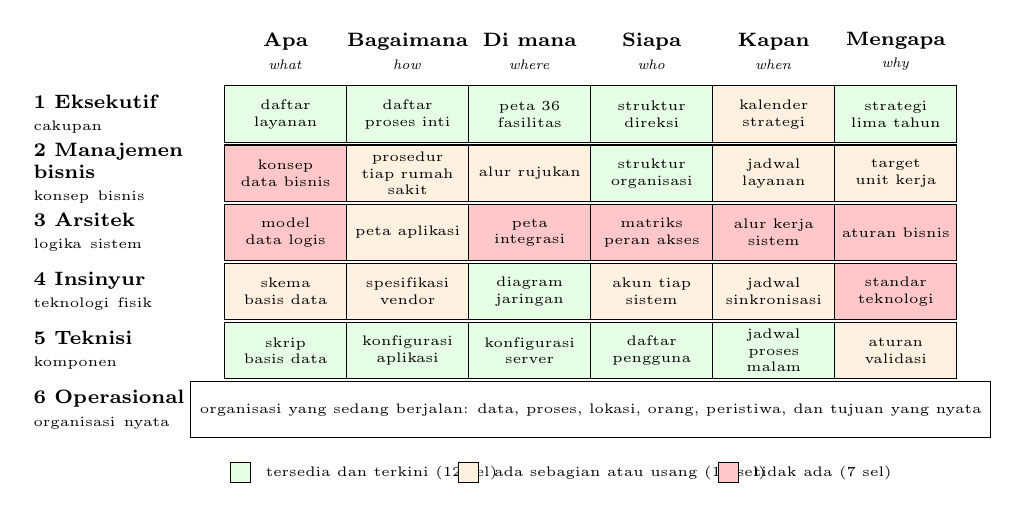
\begin{tikzpicture}[
  font=\scriptsize,
  sel/.style={draw, minimum width=1.55cm, minimum height=0.72cm, text width=1.4cm,
              align=center, font=\tiny, inner sep=1pt},
  kolom/.style={minimum width=1.55cm, minimum height=0.6cm, align=center,
                font=\scriptsize\bfseries, inner sep=1pt},
  baris/.style={minimum width=2.5cm, minimum height=0.72cm, text width=2.35cm,
                align=left, font=\scriptsize\bfseries, inner sep=1pt},
  ada/.style={sel, fill=green!10},
  sebagian/.style={sel, fill=orange!12},
  kosong/.style={sel, fill=red!22}
]
  % Judul kolom: enam kata tanya.
  \node[kolom] at (3.275,0) {Apa\\{\tiny\mdseries\textit{what}}};
  \node[kolom] at (4.825,0) {Bagaimana\\{\tiny\mdseries\textit{how}}};
  \node[kolom] at (6.375,0) {Di mana\\{\tiny\mdseries\textit{where}}};
  \node[kolom] at (7.925,0) {Siapa\\{\tiny\mdseries\textit{who}}};
  \node[kolom] at (9.475,0) {Kapan\\{\tiny\mdseries\textit{when}}};
  \node[kolom] at (11.025,0) {Mengapa\\{\tiny\mdseries\textit{why}}};

  % Baris 1: eksekutif.
  \node[baris] at (1.25,-0.8) {1 Eksekutif\\{\tiny\mdseries cakupan}};
  \node[ada] at (3.275,-0.8) {daftar layanan};
  \node[ada] at (4.825,-0.8) {daftar proses inti};
  \node[ada] at (6.375,-0.8) {peta 36 fasilitas};
  \node[ada] at (7.925,-0.8) {struktur direksi};
  \node[sebagian] at (9.475,-0.8) {kalender strategi};
  \node[ada] at (11.025,-0.8) {strategi lima tahun};

  % Baris 2: manajemen bisnis.
  \node[baris] at (1.25,-1.55) {2 Manajemen bisnis\\{\tiny\mdseries konsep bisnis}};
  \node[kosong] at (3.275,-1.55) {konsep data bisnis};
  \node[sebagian] at (4.825,-1.55) {prosedur tiap rumah sakit};
  \node[sebagian] at (6.375,-1.55) {alur rujukan};
  \node[ada] at (7.925,-1.55) {struktur organisasi};
  \node[sebagian] at (9.475,-1.55) {jadwal layanan};
  \node[sebagian] at (11.025,-1.55) {target unit kerja};

  % Baris 3: arsitek.
  \node[baris] at (1.25,-2.3) {3 Arsitek\\{\tiny\mdseries logika sistem}};
  \node[kosong] at (3.275,-2.3) {model data logis};
  \node[sebagian] at (4.825,-2.3) {peta aplikasi};
  \node[kosong] at (6.375,-2.3) {peta integrasi};
  \node[kosong] at (7.925,-2.3) {matriks peran akses};
  \node[kosong] at (9.475,-2.3) {alur kerja sistem};
  \node[kosong] at (11.025,-2.3) {aturan bisnis};

  % Baris 4: insinyur.
  \node[baris] at (1.25,-3.05) {4 Insinyur\\{\tiny\mdseries teknologi fisik}};
  \node[sebagian] at (3.275,-3.05) {skema basis data};
  \node[sebagian] at (4.825,-3.05) {spesifikasi vendor};
  \node[ada] at (6.375,-3.05) {diagram jaringan};
  \node[sebagian] at (7.925,-3.05) {akun tiap sistem};
  \node[sebagian] at (9.475,-3.05) {jadwal sinkronisasi};
  \node[kosong] at (11.025,-3.05) {standar teknologi};

  % Baris 5: teknisi.
  \node[baris] at (1.25,-3.8) {5 Teknisi\\{\tiny\mdseries komponen}};
  \node[ada] at (3.275,-3.8) {skrip basis data};
  \node[ada] at (4.825,-3.8) {konfigurasi aplikasi};
  \node[ada] at (6.375,-3.8) {konfigurasi server};
  \node[ada] at (7.925,-3.8) {daftar pengguna};
  \node[ada] at (9.475,-3.8) {jadwal proses malam};
  \node[sebagian] at (11.025,-3.8) {aturan validasi};

  % Baris 6: organisasi yang berjalan.
  \node[baris] at (1.25,-4.55) {6 Operasional\\{\tiny\mdseries organisasi nyata}};
  \node[draw, minimum width=9.3cm, minimum height=0.72cm, align=center, font=\tiny,
        fill=white] at (7.15,-4.55)
    {organisasi yang sedang berjalan: data, proses, lokasi, orang, peristiwa, dan tujuan yang nyata};

  % Keterangan warna.
  \node[draw, fill=green!10, minimum size=0.25cm] at (2.7,-5.35) {};
  \node[font=\tiny, anchor=west] at (2.9,-5.35) {tersedia dan terkini (12 sel)};
  \node[draw, fill=orange!12, minimum size=0.25cm] at (5.6,-5.35) {};
  \node[font=\tiny, anchor=west] at (5.8,-5.35) {ada sebagian atau usang (11 sel)};
  \node[draw, fill=red!22, minimum size=0.25cm] at (8.9,-5.35) {};
  \node[font=\tiny, anchor=west] at (9.1,-5.35) {tidak ada (7 sel)};
\end{tikzpicture}
